\documentclass{scrartcl}
\usepackage{geometry}
\usepackage{csquotes}
\usepackage{hyperref}
\usepackage{graphicx}
\usepackage{float}
\usepackage{subcaption}
\graphicspath{ {images/} }

\geometry{legalpaper, portrait, margin=1in}
 
\title{Harvard University, John A. Paulson School of Engineering and Applied Sciences \newline}
\subtitle{CS236r Project Update\\ Computational Results For Peer-Prediction and Crowdsourced Judgement Elicitation}
\author{Virgile Audi (vaudi@g.harvard.edu)\\
		Charles Liu (cliu02@g.harvard.edu)}

\begin{document}
 
\maketitle
\section*{Introduction}

We had for objective for this first milestone to implement in Python the basic set ups of the \emph{Crowdsourced Judgement Elicitation with Endogenous Proficiency} and \emph{Eliciting Informative Feedback: The Peer-Prediction Method} and be able to recreate the results of the paper before challenging them.

\section{Updates}
\subsection{Crowdsourced Elicitation}
A simple Python framework has been written to easily test different strategies for the agents. There is a base agent class with three functions: proficiency, has\_effort, and report each of which return a value $\in [0,1]$. Using the task assignment algorithm described in Section 5, we replicated the major results from the paper computationally, with proficiency $\geq 0.5$, has\_effort 0 and 1 for giving no effort and full effort respectively, and report 0 and 1 for reporting untruthfully and truthfully respectively.\\

Plots can be found in the Results section, including the result supporting Lemma 8 which we found most interesting: 
\begin{displayquote}
Suppose the probability of agent i using strategy (1, X) is $\delta$ and strategy $(0, r_i)$ is $1-\delta$ for each task $j \in J(i)$. Suppose i'’s potential reference raters $r_j (i)$ use strategies (1, X) and $(0, r_{r_j} (i))$ with probabilities $\epsilon_{r_j}(i)$ and $1-\epsilon_{r_j}(i)$ respectively, for each task $j \in J(i)$. If $\epsilon_{r_j}(i) > 0$ for any reference rater with proficiency $p_{r_j} (i) > \frac{1}{2}$, then agent i has a (strict) profitable deviation to $\delta'=1$, i.e., to always using strategy (1, X), for all values of $r_i \in [0,1]$
\end{displayquote}

The rewards in each scenario are scaled by 10 to see an interesting separation between strategies - as the paper states when presenting the reward formula, the scaling factor can be used to outweigh any costs incurred to the agent for completing a task. For the remainder of the project, how costs are related to effort will be the focus. In the paper their assumptiosn regarding cost are very general: they assume that costs are 0 for no effort and some constant value for full effort, though they note that all of their results apply when cost and proficiency are linearly scaled to effort. \\

This is a very unrealistic assumption - as noted towards the end of the paper a natural extension would be to introduce the concept of difficulty to particular tasks. In this scenario proficiency on a task is a function of both effort and difficulty, and costs are a function of effort (perhaps convexly). It would seem the optimal strategy would then be to give little effort on difficult tasks and focus on getting rewards for the easier tasks. The first goal would be to validate this intuition. Finally, we would like to come up with a modification for the reward formula to incentivize giving effort to more difficult problems.

\subsection{Peer Prediction}

We recall the main assumptions made in the paper:

\begin{enumerate}
\item Conditional on the product’s type, raters’ signal sare independent and identically distributed, i.e. raters have common prior
\item Raters have common knowledge of the probability of reporting a signal given a type of a product.
\end{enumerate}

The objective of this project being to relax some of these assumptions, we implemented an agent class in python that would allow for different prior distribibutions as well as personal signal probability given the particular type of a product. We also implemented the various score functions mentioned in the paper, i.e. Quadratic, Spherical and Log scoring rules.

We then wanted to verify the main proposition of the paper:

\begin{displayquote}
For any mapping r that assigns to each rater i a reference rater r i  ̸= i, and for any proper scoring rule R, truthful reporting is a strict Nash equilibrium of the simultaneous reporting game with transfers  i∗ .
\end{displayquote}

To do so, we simulated 1000 experiments where 2 agents who satisfy the assumptions presented above, reports 1000 signals over two types. We fix agent 2 to always be truthful and let agent 1 be truthful, deceitful or even adopt a randomised strategy (0.5, 0.5). As we can see on figure 4, it seems to always be better to report truthfully, even if it is only slightly more advantageous than to report using a randomised strategy. This last statement could also be invalidated with further testing and different randomised strategies.\\

We also noted an interesting results when trying to relax the second assumption stated above. For Proposition 1 to hold, we in fact need not only that  raters have common knowledge of the probability of reporting a signal given a type of a product, but also that these distributions are to be the same. To validate this new assumption, we simulated the same experiments as before, but with agents having different distributions of perception, which is in fact close to the proficiency consideration of the crowd-sourcing paper. In one case, we used an agent that was rather undecided when receiving a signal, having a 50\% chance of correctly reading the signal. In the other, we designed an agent that was very bad at identifying the type for which the second agent is actually quite good at, and keeping the second type distribution the same. Figure 6 shows that to always lie is a better strategy for agent 1, if he knows that he tends to read signals worse than his refering agent !\\ 

Next steps of this part of the project will be to focus on this issue as well as relaxing the first assumption of common priors over types.
\section{Results}
\subsection{Crowdsourced Elicitation}
\begin{figure}[H]
	\caption{Computational results of different equilibriums vs. other strategies}
	\centering
	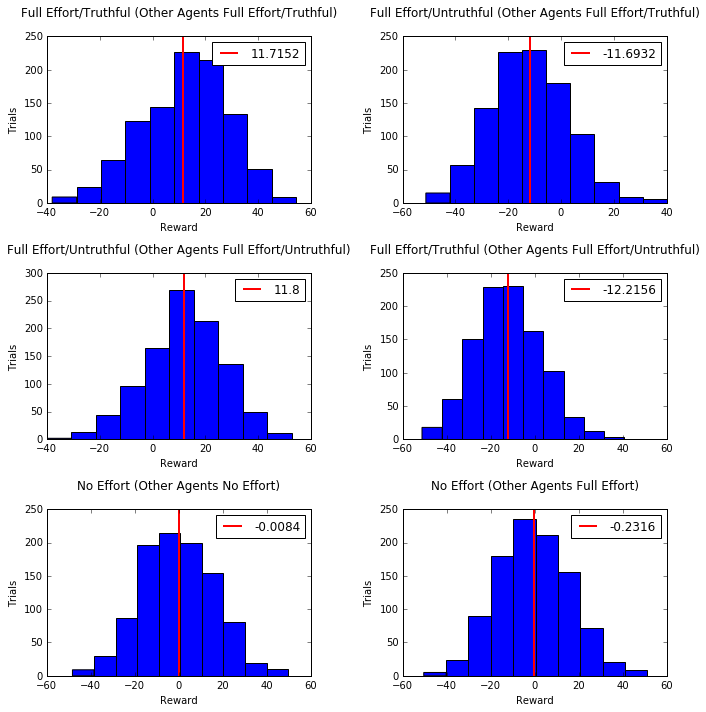
\includegraphics[width=1.0\textwidth]{cs_equilibriums}
\end{figure}
\begin{figure}[H]
	\caption{Computational results of Lemma 8}
	\centering
	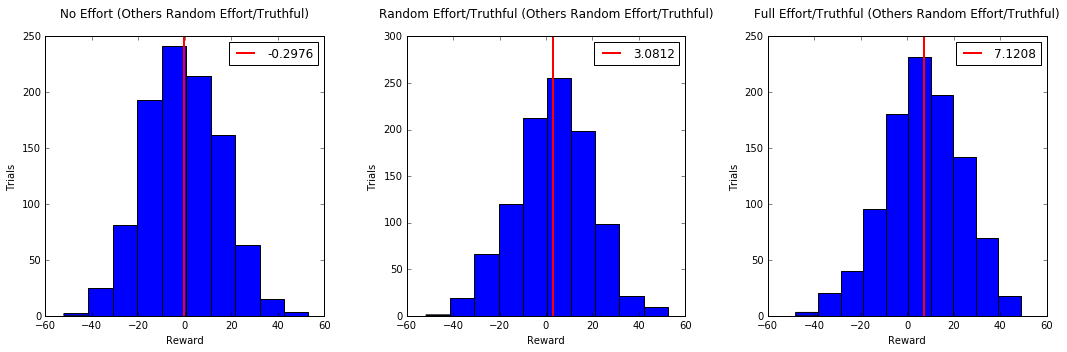
\includegraphics[width=1.0\textwidth]{cs_lemma8}
\end{figure}

\begin{figure}[H]
	\caption{Computational results of Lemma 8}
	\centering
	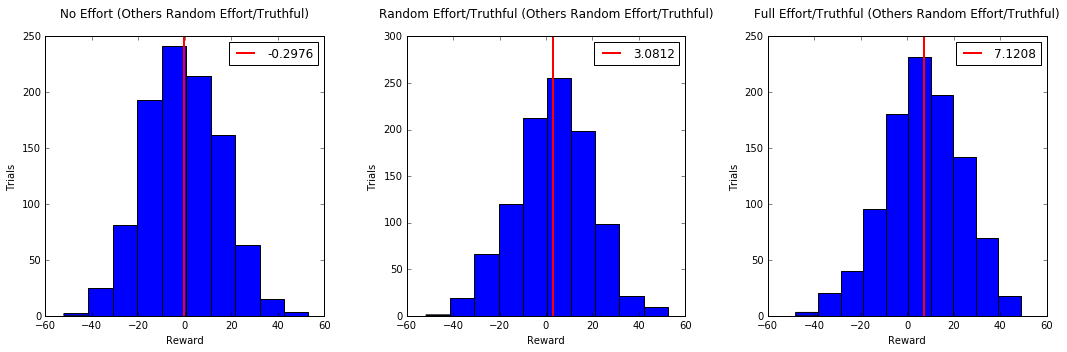
\includegraphics[width=1.0\textwidth]{cs_lemma8}
\end{figure}
\subsection{Peer Prediction}
\begin{figure}[H]
\caption{Computational verification of Property 1}
\begin{subfigure}{0.4\textwidth}
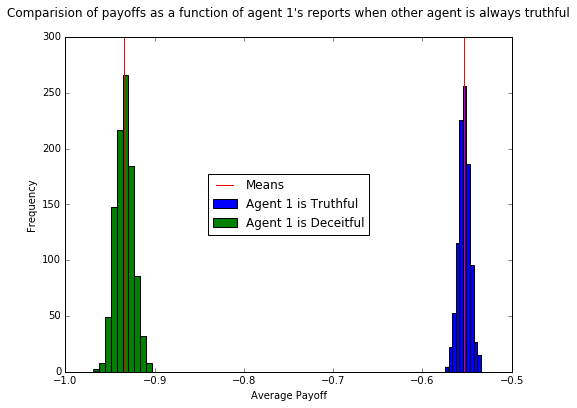
\includegraphics[scale=0.4]{pp_1}
\end{subfigure}
\hspace{0.1\textwidth}
\begin{subfigure}{0.4\textwidth}
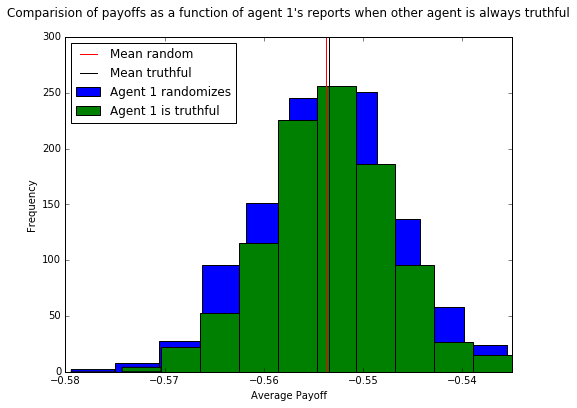
\includegraphics[scale=0.4]{rand}
\end{subfigure}
\end{figure}

\begin{figure}[H]
\caption{Relaxing Assumption 2}
\begin{subfigure}{0.4\textwidth}
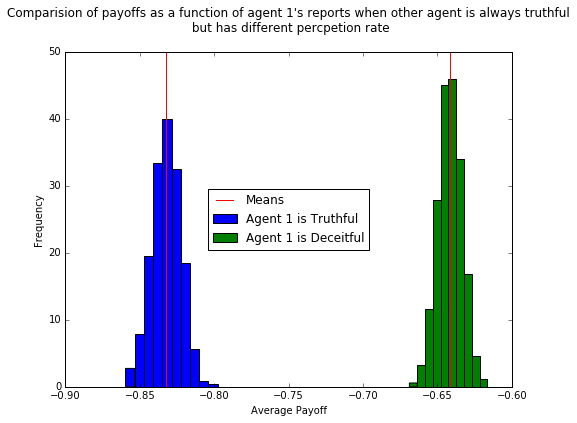
\includegraphics[scale=0.4]{pp_2}
\end{subfigure}
\hspace{0.1\textwidth}
\begin{subfigure}{0.4\textwidth}
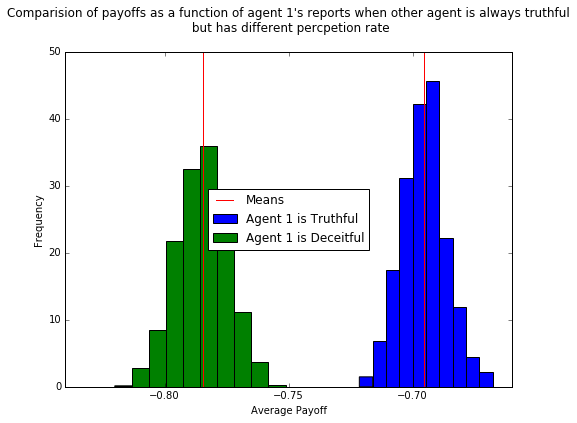
\includegraphics[scale=0.4]{pp_3}
\end{subfigure}
\end{figure}
\end{document}